\documentclass[../main.tex]{subfiles}
\graphicspath{{\subfix{../diagrams/}}}

\begin{document}

\chapter{Cryptography}

This chapter talks about cryptography and concepts related to it, We start by talking generally on cryptography then we focus on the encryption method related to our project.

\section{State of art}

Cryptography is the science of secret writing with the goal of hiding the meaning of a message.\cite{10.5555/1721909}

Cryptography itself splits into three main branches:

\begin{itemize}
\item \textbf{Symmetric Algorithms} two parties have an encryption and decryption method for which they share a
secret key. All cryptography from ancient times until 1976 was exclusively based
on symmetric methods. Symmetric ciphers are still in widespread use, especially
for data encryption and integrity check of messages.\cite{10.5555/1721909}
\end{itemize}


\begin{itemize}
\item \textbf{Asymmetric (or Public-Key) Algorithms} a user possesses a secret key as in symmetric cryptography but also a public key. Asymmetric algorithms can be used for applications
such as digital signatures and key establishment, and also for classical data encryption.\cite{10.5555/1721909}
\end{itemize}


\begin{itemize}
\item \textbf{Cryptographic Protocols} Roughly speaking, crypto protocols deal with the application of cryptographic algorithms. Symmetric and asymmetric algorithms can be viewed as building blocks with which applications such as secure Internet communication can be realized. The Transport Layer Security (TLS) scheme,
which is used in every Web browser, is an example of a cryptographic protocol.\cite{10.5555/1721909}
\end{itemize}

We will focus on the Symmetric Cryptography as it is related to our project.

\subsection{Symmetric Cryptography}


Symmetric cryptographic schemes are also referred to as symmetric-key, secret-key,
and single-key schemes or algorithms. Symmetric cryptography is best introduced
with an easy to understand problem: There are two users, Alice and Bob, who want
to communicate over an insecure channel\cite{10.5555/1721909} (Fig \ref{fig:cryp1})

\begin{figure}[h]
\centering
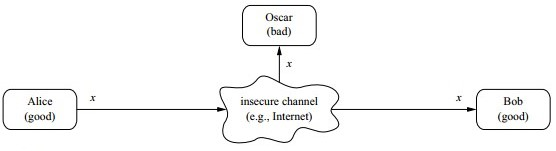
\includegraphics[width=15cm]{diagrams/cryp1.jpg}

\caption{Communication over an insecure channel}
\label{fig:cryp1}
\end{figure}

In this situation, symmetric cryptography offers a powerful solution: Alice encrypts her message x using a symmetric algorithm, yielding the ciphertext y. Bob
receives the ciphertext and decrypts the message. Decryption is, thus, the inverse
process of encryption (Fig. \ref{fig:cryp2}). What is the advantage? If we have a strong encryption algorithm, the ciphertext will look like random bits to Oscar and will contain
no information whatsoever that is useful to him.\cite{10.5555/1721909}

\begin{figure}[h]
\centering
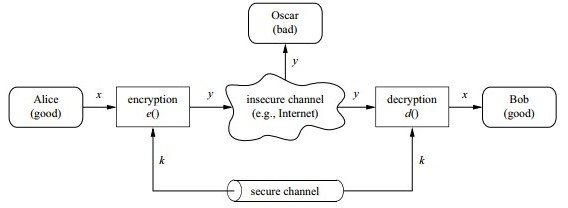
\includegraphics[width=15cm]{diagrams/cryp2.jpg}

\caption{Symmetric-key cryptosystem}
\label{fig:cryp2}
\end{figure}

The variables x, y and k in Fig. \ref{fig:cryp2} are important in cryptography and have special
names:

 x is called plaintext or cleartext,
 
 y is called ciphertext,
 
 k is called the key,
 
 the set of all possible keys is called the key space.

\section{Used Cryptographic Algorithm}

\subsection{The Advanced Encryption Standard (AES)}
The Advanced Encryption Standard (AES) is the most widely used symmetric cipher
today. The AES block cipher is also mandatory in several industry standards
and is used in many commercial systems. Among the commercial standards that
include AES are the Internet security standard IPsec, TLS, the Wi-Fi encryption
standard IEEE 802.11i, the secure shell network protocol SSH (Secure Shell), the
Internet phone Skype and numerous security products around the world. To date,
there are no attacks better than brute-force known against AES.\cite{10.5555/1721909}

\subsubsection{Overview of the AES Algorithm}

The AES cipher is almost identical to the block cipher Rijndael. The Rijndael block
and key size vary between 128, 192 and 256 bits. However, the AES standard only
calls for a block size of 128 bits. Hence, only Rijndael with a block length of 128
bits is known as the AES algorithm. In the remainder of this chapter, we only discuss
the standard version of Rijndael with a block length of 128 bits.\cite{10.5555/1721909}

\begin{figure}[h]
\centering
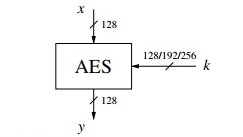
\includegraphics[width=10cm]{diagrams/cryp3.jpg}

\caption{AES input/output parameters}
\label{fig:cryp3}
\end{figure}
AES, encrypts all 128 bits in one iteration. This is
one reason why it has a comparably small number of rounds.
AES consists of so-called layers. Each layer manipulates all 128 bits of the data
path. The data path is also referred to as the state of the algorithm. There are only
three different types of layers. Each round, with the exception of the first, consists
of all three layers as shown in Fig. \ref{fig:cryp4}: the plaintext is denoted as x, the ciphertext
as y and the number of rounds as nr. Moreover, the last round nr does not make
use of the MixColumn transformation, which makes the encryption and decryption
scheme symmetric.\cite{10.5555/1721909}
\begin{figure}[h]
\centering
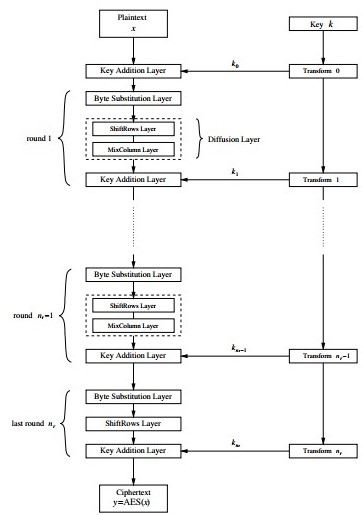
\includegraphics[width=11cm]{diagrams/cryp4.jpg}

\caption{AES encryption block diagram}
\label{fig:cryp4}
\end{figure}
We continue with a brief description of the layers:

\textbf{Key Addition layer} A 128-bit round key, or subkey, which has been derived from
the main key in the key schedule, is XORed to the state.

\textbf{Byte Substitution layer} (S-Box) Each element of the state is nonlinearly transformed using lookup tables with special mathematical properties.This introduces
confusion to the data, i.e., it assures that changes in individual state bits propagate
quickly across the data path.

\textbf{Diffusion layer} It provides diffusion over all state bits. It consists of two sublayers,
both of which perform linear operations:
 The ShiftRows layer permutes the data on a byte level.
 The MixColumn layer is a matrix operation which combines (mixes) blocks of four bytes.


\subsection{Internal Structure of AES}

In the following, we examine the internal structure of AES. Figure \ref{fig:cryp5} shows the
graph of a single AES round. The 16-byte input A0,...,A15 is fed byte-wise into the S-Box. The 16-byte output B0,...,B15 is permuted byte-wise in the ShiftRows layer
and mixed by the MixColumn transformation c(x). Finally, the 128-bit subkey ki is
XORed with the intermediate result. We note that AES is a byte-oriented cipher.\cite{10.5555/1721909}

\begin{figure}[h]
\centering
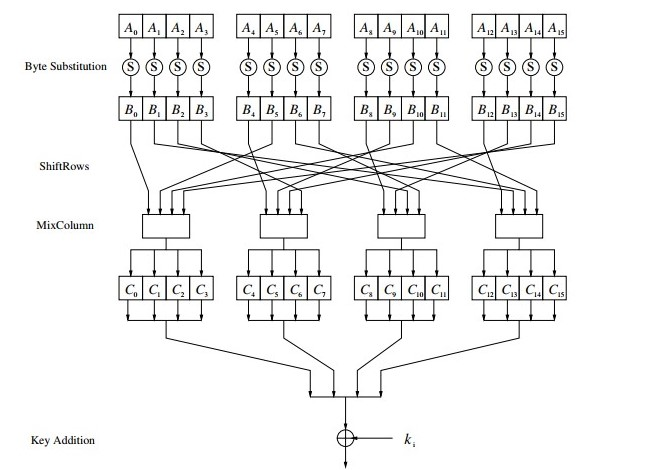
\includegraphics[width=13cm]{diagrams/cryp5.jpg}

\caption{AES round function for rounds 1,2,...,n-1}
\label{fig:cryp5}
\end{figure}

In order to understand how the data moves through AES, we first imagine that the
state A (i.e., the 128-bit data path) consisting of 16 bytes A0,A1,...,A15 is arranged
in a four-by-four byte matrix:
\begin{figure}[h]
\centering
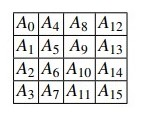
\includegraphics[width=3.5cm]{diagrams/cryp6.jpg}
\end{figure}
As we will see in the following, AES operates on elements, columns or rows of
the current state matrix. Similarly, the key bytes are arranged into a matrix with four
rows and four (128-bit key), six (192-bit key) or eight (256-bit key) columns.

\subsubsection{Byte Substitution Layer}
The Byte Substitution layer can be viewed as a row of 16 parallel S-Boxes, each with 8 input and output bits.
In the layer, each state byte Ai is replaced, i.e.,
substituted, by another byte Bi.

The S-Box is the only nonlinear element of AES, i.e., it holds that ByteSub(A) + ByteSub(B) = ByteSub(A + B) for two states A and B. The S-Box substitution is a
bijective mapping, i.e., each of the 28 = 256 possible input elements is one-to-one
mapped to one output element. This allows us to uniquely reverse the S-Box, which
is needed for decryption. In software implementations the S-Box is usually realized
as a 256-by-8 bit lookup table with fixed entries,\cite{10.5555/1721909} as given in Fig \ref{fig:cryp8}.

\begin{figure}[h]
\centering
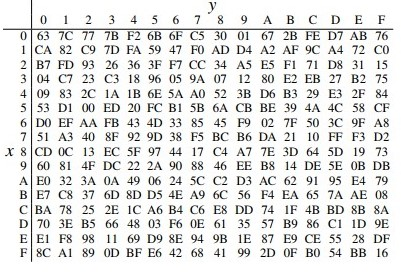
\includegraphics[width=13cm]{diagrams/cryp8.jpg}

\caption{AES S-Box: Substitution values in hexadecimal notation for input byte (xy)}
\label{fig:cryp8}
\end{figure}
Let’s assume the input byte to the S-Box is Ai = (C2)hex, then the
substituted value is
\begin{center} 
S((C2)hex) = (25)hex
\end{center}

\subsubsection{Diffusion Layer}
In AES, the Diffusion layer consists of two sublayers, the ShiftRows transformation
and the MixColumn transformation. We recall that diffusion is the spreading of the
influence of individual bits over the entire state. Unlike the nonlinear S-Box, the diffusion layer performs a linear operation on state matrices A,B, i.e., DIFF(A) +
DIFF(B) = DIFF(A + B).\cite{10.5555/1721909}

\subsubsection{ShiftRows Sublayer}
The ShiftRows transformation cyclically shifts the second row of the state matrix
by three bytes to the right, the third row by two bytes to the right and the fourth
row by one byte to the right. The first row is not changed by the ShiftRows transformation. The purpose of the ShiftRows transformation is to increase the diffusion
properties of AES. If the input of the ShiftRows sublayer is given as a state matrix
B = (B0,B1,...,B15):
\begin{figure}[h]
\centering
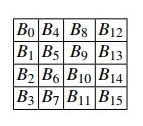
\includegraphics[width=4cm]{diagrams/cryp10.jpg}
\end{figure}
the output is the new state:
\begin{figure}[h]
\centering
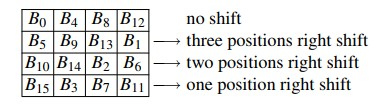
\includegraphics[width=10cm]{diagrams/cryp11.jpg}
\end{figure}

\subsubsection{MixColumn Sublayer}
The MixColumn step is a linear transformation which mixes each column of the
state matrix. Since every input byte influences four output bytes, the MixColumn
operation is the major diffusion element in AES. The combination of the ShiftRows
and MixColumn layer makes it possible that after only three rounds every byte of
the state matrix depends on all 16 plaintext bytes.
In the following, we denote the 16-byte input state by B and the 16-byte output
state by C:
\begin{figure}[h]
\centering
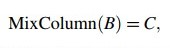
\includegraphics[width=4cm]{diagrams/cryp12.jpg}
\end{figure}

where B is the state after the ShiftRows operation.
Now, each 4-byte column is considered as a vector and multiplied by a fixed
4 × 4 matrix. The matrix contains constant entries.
we show how the first four output
bytes are computed:
\begin{figure}[h]
\centering
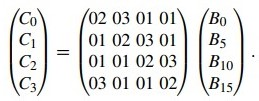
\includegraphics[width=7cm]{diagrams/cryp13.jpg}
\end{figure}
The second column of output bytes (C4,C5,C6,C7) is computed by multiplying
the four input bytes (B4,B9,B14,B3) by the same constant matrix, and so on. 

\subsubsection{Key Addition Layer}
The two inputs to the Key Addition layer are the current 16-byte state matrix and
a subkey which also consists of 16 bytes (128 bits). The two inputs are combined
through a bitwise XOR operation. 

\subsubsection{Key Schedule}
The key schedule takes the original input key (of length 128, 192 or 256 bit) and
derives the subkeys used in AES. Note that an XOR addition of a subkey is used
both at the input and output of AES. This process is sometimes referred to as key
whitening. The number of subkeys is equal to the number of rounds plus one, due
to the key needed for key whitening in the first key addition layer, cf. Fig. \ref{fig:cryp4}.
Thus, for the key length of 128 bits, the number of rounds is nr = 10, and there are
11 subkeys, each of 128 bits. The AES with a 192-bit key requires 13 subkeys of
length 128 bits, and AES with a 256-bit key has 15 subkeys. The AES subkeys are
computed recursively, i.e., in order to derive subkey ki, subkey ki-1 must be known,
etc.\cite{10.5555/1721909}

The AES key schedule is word-oriented, where 1 word = 32 bits. Subkeys are
stored in a key expansion array W that consists of words. There are different key
schedules for the three different AES key sizes of 128, 192 and 256 bit, which are
all fairly similar. We introduce the three key schedules in the following.
We will focus only on size 128 as it is related to our project.\cite{10.5555/1721909}
\subsubsection{Key Schedule for 128-Bit Key AES}
\begin{figure}[h]
\centering
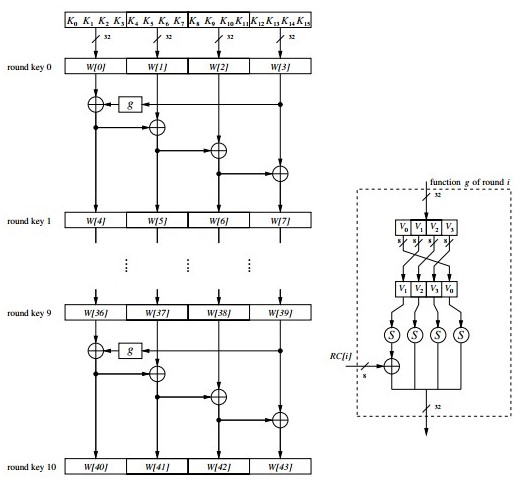
\includegraphics[width=11cm]{diagrams/cryp14.jpg}

\caption{AES key schedule for 128-bit key size}
\label{fig:cryp14}
\end{figure}
The ll subkeys are stored in a key expansion array with the elements W[0],...,W[43].
The subkeys are computed as depicted in Fig. \ref{fig:cryp14}. The elements K0,...,K15 denote
the bytes of the original AES key.
First, we note that the first subkey k0 is the original AES key, i.e., the key is
copied into the first four elements of the key array W. The other array elements are computed as follows. As can be seen in the figure, the leftmost word of a subkey
W[4i], where i = 1,...,10, is computed as:
\begin{center} 
W[4i] = W[4(i-1)]+g(W[4i-1]).
\end{center}
Here g() is a nonlinear function with a four-byte input and output. The remaining
three words of a subkey are computed recursively as:
\begin{center} 
W[4i+ j] = W[4i+ j -1] +W[4(i-1)+ j],
\end{center}
where i = 1,...,10 and j = 1,2,3. The function g() rotates its four input bytes,
performs a byte-wise S-Box substitution, and adds a round coefficient RC to it.

\subsection{Decryption}
In AES decryption all layers must be inverted, i.e., the Byte Substitution layer becomes the Inv Byte Substitution layer,
the ShiftRows layer becomes the Inv ShiftRows layer, and the MixColumn layer
becomes Inv MixColumn layer. However, as we will see, it turns out that the inverse
layer operations are fairly similar to the layer operations used for encryption. In addition, the order of the subkeys is reversed, i.e., we need a reversed key schedule. A
block diagram of the decryption function is shown in Fig. \ref{fig:cryp15}.
\begin{figure}[h]
\centering
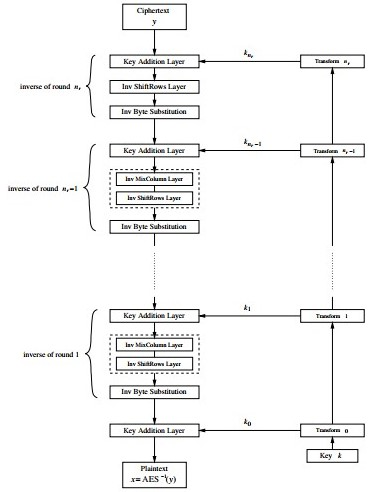
\includegraphics[width=12cm]{diagrams/cryp15.jpg}

\caption{AES decryption block diagram}
\label{fig:cryp15}
\end{figure}

Since the last encryption round does not perform the MixColumn operation, the
first decryption round also does not contain the corresponding inverse layer. All
other decryption rounds, however, contain all AES layers. In the following, we discuss the inverse layers of the general AES decryption round (Fig. \ref{fig:cryp16}). Since the XOR operation is its own inverse, the key addition layer in the decryption mode is
the same as in the encryption mode: it consists of a row of plain XOR gates.

\begin{figure}[h]
\centering
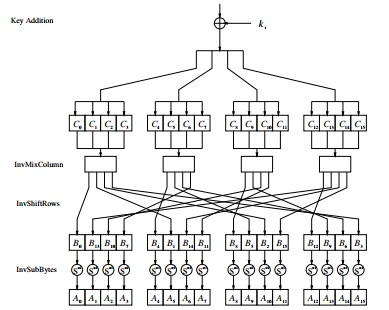
\includegraphics[width=10cm]{diagrams/cryp16.jpg}

\caption{AES decryption round function 1,2,...,nr -1}
\label{fig:cryp16}
\end{figure}

\subsubsection{Inverse MixColumn Sublayer}
After the addition of the subkey, the inverse MixColumn step is applied to the state
(again, the exception is the first decryption round). In order to reverse the MixColumn operation, the inverse of its matrix must be used. The input is a 4-byte column
of the State C which is multiplied by the inverse 4×4 matrix. The matrix contains
constant entries. 
\begin{figure}[h]
\centering
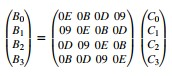
\includegraphics[width=6cm]{diagrams/cryp17.jpg}
\end{figure}

The second column of output bytes (B4,B5,B6,B7) is computed by multiplying the
four input bytes (C4,C5,C6,C7) by the same constant matrix, and so on.

\subsubsection{Inverse ShiftRows Sublayer}
In order to reverse the ShiftRows operation of the encryption algorithm, we must
shift the rows of the state matrix in the opposite direction. The first row is not
changed by the inverse ShiftRows transformation. If the input of the ShiftRows
sublayer is given as a state matrix B = (B0,B1,...,B15):
\begin{figure}[h]
\centering
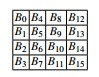
\includegraphics[width=3cm]{diagrams/cryp18.jpg}
\end{figure}
the inverse ShiftRows sublayer yields the output:
\begin{figure}[h]
\centering
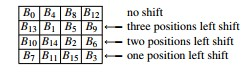
\includegraphics[width=8cm]{diagrams/cryp19.jpg}
\end{figure}
\subsubsection{Inverse Byte Substitution Layer}
The inverse S-Box is used when decrypting a ciphertext. Since the AES S-Box is
a bijective, i.e., a one-to-one mapping, it is possible to construct an inverse S-Box
such that:
\begin{center} 
Ai = Sinv(Bi) = Sinv(S(Ai)),
\end{center}
where Ai and Bi are elements of the state matrix. The entries of the inverse S-Box
are given in Fig.(\ref{fig:cryp20}).
\begin{figure}[h]
\centering
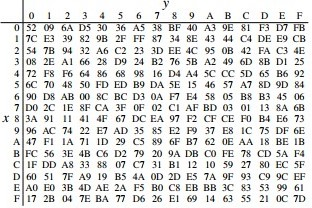
\includegraphics[width=10cm]{diagrams/cryp20.jpg}

\caption{Inverse AES S-Box: Substitution values in hexadecimal notation for input byte (xy)}
\label{fig:cryp20}
\end{figure}
\subsubsection{Decryption Key Schedule}
Since decryption round one needs the last subkey, the second decryption round
needs the second-to-last subkey and so on, we need the subkey in reversed order
as shown in Fig. \ref{fig:cryp15}. In practice this is mainly achieved by computing the entire
key schedule first and storing all 11, 13 or 15 subkeys, depending on the number or rounds AES is using (which in turn depends on the three key lengths supported by
AES). This precomputation adds usually a small latency to the decryption operation
relative to encryption.
\end{document}

